% -------------------------------------------------------------------------
\subsection{Point forecasting and horizon decomposition}
\label{app:point}

Table~\ref{tab:point} gives the complete point comparison retained for
continuity with the intermittent-demand literature. Rankings exclude the
deliberately degenerate Zero and Naive-last rows. \EBB{} takes six of
ten MAE/RMSSE cells and is top two on seven, but the result is not uniform:
classical methods retain several point-metric wins, and Zero attains the
lowest MAE on Online Retail, Carparts, and RAF. This is why the main text
uses point accuracy as a secondary diagnostic.

\begin{table*}[t]
\centering
\caption{Point forecasting across the five panels (lower is better;
bold best and underline second among non-degenerate methods). Degenerate
rows are shown as metric diagnostics and excluded from ranking.}
\label{tab:point}
\small
\setlength{\tabcolsep}{3.4pt}
\begin{tabular}{lcc@{\hspace{10pt}}cc@{\hspace{10pt}}cc@{\hspace{10pt}}cc@{\hspace{10pt}}cc}
\toprule
 & \multicolumn{2}{c}{Online Retail} & \multicolumn{2}{c}{M5} & \multicolumn{2}{c}{Auto} & \multicolumn{2}{c}{Carparts} & \multicolumn{2}{c}{RAF}\\
\cmidrule(lr){2-3}\cmidrule(lr){4-5}\cmidrule(lr){6-7}\cmidrule(lr){8-9}\cmidrule(lr){10-11}
Model & MAE & RMSSE & MAE & RMSSE & MAE & RMSSE & MAE & RMSSE & MAE & RMSSE\\
\midrule
CrostonClassic & 6.3294 & 5.1051 & 1.2345 & 2.3539 & 3.4056 & 1.1488 & 0.6792 & 1.0981 & 2.7315 & 1.6280\\
CrostonSBA & 6.1953 & 5.0692 & 1.2076 & 2.3517 & \secondbest{3.3325} & \secondbest{1.1451} & 0.6628 & 1.0935 & 2.6520 & 1.6272\\
TSB & \secondbest{5.5736} & 4.8031 & 1.2672 & 2.3612 & 3.6587 & 1.2066 & \best{0.5396} & 1.0156 & \best{2.1660} & 1.6570\\
TSB-tuned & 5.6318 & 4.7985 & \best{1.1932} & \secondbest{2.3137} & 3.3917 & 1.1452 & \best{0.5396} & 1.0156 & \secondbest{2.2447} & 1.6408\\
ADIDA & 5.6860 & \secondbest{4.7967} & 1.2274 & 2.3398 & 3.4079 & 1.1545 & 0.5556 & 1.0244 & 2.2977 & \secondbest{1.6245}\\
IMAPA & 5.7000 & 4.7970 & 1.2317 & 2.3280 & 3.4143 & 1.1555 & \secondbest{0.5524} & 1.0126 & 2.2850 & 1.6259\\
AutoARIMA & 6.5494 & 4.8175 & 1.2283 & 2.3169 & 3.4417 & 1.1745 & 0.5822 & \secondbest{1.0105} & 2.3153 & 1.6262\\
AutoTheta & 8.2862 & 4.8550 & 1.2988 & 2.3143 & 3.7490 & 1.2215 & 0.5704 & \best{0.9966} & 2.3687 & 1.6399\\
\midrule
Zero & 4.7549 & 4.8089 & 1.2995 & 2.4629 & 4.1444 & 1.4454 & 0.3867 & 1.0949 & 1.1717 & 1.6345\\
Naive-last & 6.0570 & 4.8324 & 1.3750 & 2.5450 & 4.3529 & 1.3818 & 0.5399 & 1.1408 & 1.8340 & 1.7644\\
\midrule
\EBB{} (ours) & \best{5.5325} & \best{4.7901} & \secondbest{1.2032} & \best{2.2938} & \best{3.2145} & \best{1.1374} & 0.5726 & 1.0120 & 2.3874 & \best{1.6245}\\
\bottomrule
\end{tabular}
\end{table*}

\begin{figure}[t]
\centering
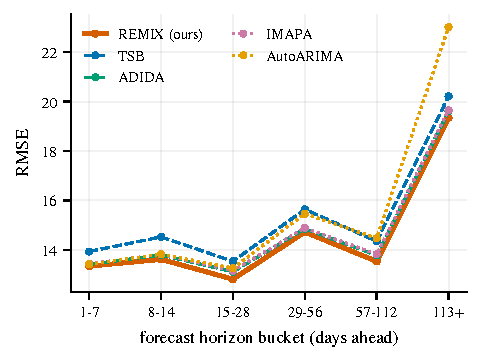
\includegraphics[width=0.93\linewidth]{figs/horizon_decomp.pdf}
\caption{Online Retail RMSE by fixed-origin forecast-horizon bucket.
\EBB{} is lowest in every bucket, so the aggregate result is not
created by averaging only over distant horizons. MAE differences among
the leading methods are within $1$--$2\%$ by bucket.}
\label{fig:horizon}
\end{figure}

The selected $(g,w)$ pairs are: Online Retail (global, $0.95$), M5
(mixture, $0.95$), Auto (global, $0.99$), Carparts (global, $0.90$), and
RAF (mixture, $0.997$). On three of the five panels the margins between
pooling structures on the internal validation surface are under a tenth
of a percent, so the structure component of these pairs should be read as
Section~\ref{sec:leverage} reads it: the selector avoids poor structural
corners, and no winner is announced where the surface does not resolve
one.

\subsection{Selector diagnostics}
\label{sec:selector-diagnostics}
\label{app:selector-diagnostics}

The selection surface is locally flat near its optimum: on Online Retail
the best seven candidates span all three pooling structures and lie within
$0.51\%$ of one another in validation SPL. Section~\ref{sec:leverage}
reports the credibility leverage and refinement gains that accompany each
selected pair, and Figure~\ref{fig:refinement-leverage} places them
against the controlled panels. The selector is useful for choosing a
discount and for avoiding poor structural corners; the winning pooling
structure on a panel whose candidates lie within a tenth of a percent
should not be read as a scientific taxonomy. Per-panel selection surfaces
are released with the code.

\begin{table*}[t]
\centering
\caption{Full Online Retail ablation corresponding to
Table~\ref{tab:ablation}. Each row is an independent run; ``auto'' denotes
its own internal discount selection. TSB has no native predictive
distribution. Lower is better.}
\label{tab:ablation-full}
\small
\setlength{\tabcolsep}{5.0pt}
\begin{tabular}{llrrrrrr}
\toprule
Pooling & Forget & MAE & RMSE & RMSSE & SPL & SPL$_{90}$ & AIW\\
\midrule
none (TSB) & fixed & 5.5736 & 18.7272 & 4.8031 & --- & --- & ---\\
global & off & 5.7623 & \best{17.6892} & \best{4.7851} & 0.8899 & 1.5306 & 10.51\\
taxonomy & off & 5.7663 & \secondbest{17.6930} & \secondbest{4.7875} & 0.8897 & 1.5299 & 10.56\\
learned & off & 5.8126 & 17.7064 & 4.7876 & 0.8905 & 1.5336 & 10.79\\
global & auto ($.95$) & \best{5.5325} & 17.8386 & 4.7901 & \secondbest{0.8849} & \secondbest{1.5268} & \best{9.25}\\
taxonomy & auto ($.95$) & \secondbest{5.5624} & 17.8421 & 4.7897 & \best{0.8846} & \best{1.5254} & 9.43\\
learned & auto ($.95$) & 5.6925 & 17.8765 & 4.7902 & 0.8869 & 1.5343 & 10.69\\
\bottomrule
\end{tabular}
\end{table*}

\subsection{Walk-forward point results and protocol}
\label{app:walkforward}

\begin{table}[t]
\centering
\caption{Online Retail point forecasting under strict seven-day
walk-forward updates. The hierarchical rows differ in their
initialization discount and pooling structure.}
\label{tab:walkforward}
\small
\setlength{\tabcolsep}{5pt}
\begin{tabular}{lccc}
\toprule
Model & MAE & RMSE & RMSSE\\
\midrule
CrostonClassic & 5.692 & 16.937 & 4.854\\
CrostonSBA & 5.586 & 16.931 & 4.836\\
TSB & 5.434 & 17.754 & 4.815\\
ADIDA & \best{5.320} & \best{16.728} & \secondbest{4.637}\\
IMAPA & \secondbest{5.332} & \secondbest{16.745} & \best{4.632}\\
AutoARIMA & 5.482 & 16.904 & 5.105\\
AutoTheta & 5.394 & 16.836 & 4.735\\
\midrule
Stationary hierarchy ($w=1$) & 5.586 & 17.260 & 4.725\\
Forgetting hierarchy (tax., $.95$) & 5.411 & 17.059 & 4.682\\
\EBB{} (selected global, $.95$) & 5.421 & 17.188 & 4.696\\
\bottomrule
\end{tabular}
\end{table}

\begin{table*}[t]
\centering
\caption{Full Online Retail walk-forward SPL at all five quantiles and on average,
with marginal (Cov@80) and positive-demand (Cov$^{+}$@80) coverage and
average interval width (AIW). CP and ACI wrappers refit each of the 36 seven-day blocks; AutoARIMA, AutoTheta, iETS, and TweedieGP refit every four blocks; \EBB{} updates sufficient statistics each block. The zero row is excluded from ranking.}
\label{tab:wfprob-full}
\small
\setlength{\tabcolsep}{4.2pt}
\begin{tabular}{lrrrrrrrrr}
\toprule
Model & q10 & q25 & q50 & q75 & q90 & Mean & Cov@80 & Cov$^{+}$@80 & AIW\\
\midrule
AutoARIMA & 0.259 & 0.572 & 1.197 & 1.763 & 1.522 & 1.063 & 0.933 & 0.762 & 16.58\\
AutoTheta & 0.233 & 0.584 & 1.276 & 1.717 & 1.484 & 1.059 & 0.931 & 0.765 & 16.43\\
iETS & 0.236 & 0.505 & 1.302 & 1.562 & 1.940 & 1.109 & 0.598 & 0.166 & 19.74\\
CP-Croston & 0.341 & 0.778 & 1.364 & 1.745 & 2.632 & 1.372 & 0.793 & 0.478 & 5.66\\
CP-SBA & 0.334 & 0.762 & 1.343 & 1.725 & 2.722 & 1.377 & 0.793 & 0.481 & 5.75\\
CP-TSB & 0.451 & 0.899 & 1.289 & 1.385 & 2.842 & 1.373 & 0.795 & 0.468 & 5.71\\
CP-ADIDA & 0.277 & 0.627 & 1.050 & \secondbest{1.319} & 2.514 & 1.158 & 0.791 & 0.473 & 5.47\\
CP-IMAPA & 0.292 & 0.660 & 1.083 & 1.329 & 2.522 & 1.177 & 0.791 & 0.471 & 5.47\\
ACI-ADIDA & 0.186 & 0.468 & \best{0.909} & 1.324 & 1.668 & 0.911 & 0.904 & 0.646 & 19.67\\
ACI-TSB & 0.189 & 0.482 & 0.948 & 1.384 & 1.710 & 0.943 & 0.903 & 0.641 & 21.21\\
TweedieGP & \secondbest{0.183} & \secondbest{0.458} & 0.917 & 1.326 & \best{1.379} & \best{0.853} & 0.924 & 0.709 & 13.03\\
Zero (diagnostic) & 0.183 & 0.458 & 0.916 & 1.374 & 1.649 & 0.916 & 0.740 & 0.000 & 0.00\\
\midrule
\EBB{} & 0.183 & 0.458 & \secondbest{0.910} & \best{1.319} & \secondbest{1.400} & \secondbest{0.854} & 0.901 & 0.621 & 10.31\\
ACI-\EBB{} & \best{0.183} & \best{0.458} & 0.915 & 1.423 & 1.562 & 0.908 & 0.913 & 0.665 & 19.55\\
\EBB{} (rule) & 0.183 & 0.458 & 0.910 & 1.319 & 1.400 & 0.854 & 0.901 & 0.621 & 10.31\\
\bottomrule
\end{tabular}
\end{table*}

\begin{table*}[t]
\centering
\caption{Full Carparts walk-forward SPL at all five quantiles and on average,
with marginal (Cov@80) and positive-demand (Cov$^{+}$@80) coverage and
average interval width (AIW). Every baseline refits each of the six monthly blocks; \EBB{} updates sufficient statistics. The zero row is excluded from ranking.}
\label{tab:wf-carparts-full}
\small
\setlength{\tabcolsep}{4.2pt}
\begin{tabular}{lrrrrrrrrr}
\toprule
Model & q10 & q25 & q50 & q75 & q90 & Mean & Cov@80 & Cov$^{+}$@80 & AIW\\
\midrule
AutoARIMA & 0.150 & 0.282 & 0.537 & 0.643 & 0.484 & 0.419 & 0.886 & 0.620 & 1.63\\
AutoTheta & 0.120 & 0.253 & 0.523 & 0.657 & 0.474 & 0.406 & 0.902 & 0.678 & 1.80\\
iETS & 0.272 & 0.368 & 0.493 & 0.532 & 0.515 & 0.436 & 0.442 & 0.411 & 1.17\\
CP-Croston & 0.099 & 0.245 & 0.480 & 0.614 & 0.539 & 0.395 & 0.847 & 0.580 & 1.39\\
CP-SBA & 0.098 & 0.242 & 0.475 & 0.611 & 0.538 & 0.393 & 0.847 & 0.581 & 1.37\\
CP-TSB & 0.141 & 0.301 & 0.487 & 0.513 & 0.476 & 0.384 & 0.834 & 0.551 & 1.27\\
CP-ADIDA & 0.096 & 0.230 & 0.411 & 0.529 & 0.488 & 0.351 & 0.829 & 0.593 & 1.28\\
CP-IMAPA & 0.101 & 0.235 & 0.413 & 0.518 & 0.479 & 0.349 & 0.830 & 0.581 & 1.27\\
ACI-ADIDA & 0.088 & 0.221 & 0.406 & 0.517 & 0.477 & 0.342 & 0.870 & 0.604 & 1.38\\
TweedieGP & 0.075 & 0.188 & 0.375 & 0.490 & \best{0.433} & \best{0.312} & 0.931 & 0.662 & 1.46\\
Zero (diagnostic) & 0.075 & 0.187 & 0.374 & 0.560 & 0.672 & 0.374 & 0.795 & 0.000 & 0.00\\
\midrule
\EBB{} & \secondbest{0.075} & \secondbest{0.187} & \secondbest{0.372} & \secondbest{0.481} & 0.458 & 0.315 & 0.932 & 0.669 & 1.42\\
ACI-\EBB{} & \best{0.075} & \best{0.187} & \best{0.371} & \best{0.480} & \secondbest{0.452} & \secondbest{0.313} & 0.934 & 0.676 & 1.41\\
\EBB{} (rule) & 0.075 & 0.187 & 0.372 & 0.481 & 0.458 & 0.315 & 0.932 & 0.669 & 1.42\\
\bottomrule
\end{tabular}
\end{table*}

\begin{table*}[t]
\centering
\caption{Full Auto walk-forward SPL at all five quantiles and on average,
with marginal (Cov@80) and positive-demand (Cov$^{+}$@80) coverage and
average interval width (AIW). Every baseline refits each of the six monthly blocks; \EBB{} updates sufficient statistics. The zero row is excluded from ranking.}
\label{tab:wf-auto-full}
\small
\setlength{\tabcolsep}{4.2pt}
\begin{tabular}{lrrrrrrrrr}
\toprule
Model & q10 & q25 & q50 & q75 & q90 & Mean & Cov@80 & Cov$^{+}$@80 & AIW\\
\midrule
AutoARIMA & 0.141 & 0.313 & 0.447 & 0.405 & 0.263 & 0.314 & 0.778 & 0.799 & 8.73\\
AutoTheta & 0.152 & 0.320 & 0.460 & 0.418 & 0.262 & 0.322 & 0.780 & 0.825 & 9.64\\
iETS & 0.172 & 0.312 & 0.435 & 0.423 & 0.301 & 0.329 & 0.564 & 0.690 & 7.33\\
CP-Croston & 0.148 & 0.307 & 0.437 & 0.402 & 0.296 & 0.318 & 0.801 & 0.802 & 5.97\\
CP-SBA & 0.146 & 0.304 & 0.434 & 0.404 & 0.301 & 0.318 & 0.800 & 0.803 & 6.01\\
CP-TSB & 0.155 & 0.321 & 0.458 & 0.414 & 0.301 & 0.330 & 0.808 & 0.799 & 5.97\\
CP-ADIDA & 0.149 & 0.307 & 0.437 & 0.400 & 0.295 & 0.318 & 0.802 & 0.802 & 5.92\\
CP-IMAPA & 0.149 & 0.307 & 0.437 & 0.400 & 0.295 & 0.318 & 0.802 & 0.802 & 5.92\\
ACI-ADIDA & 0.139 & 0.305 & 0.438 & 0.401 & 0.290 & 0.315 & 0.830 & 0.822 & 6.74\\
TweedieGP & 0.122 & 0.279 & \secondbest{0.418} & \best{0.389} & \best{0.254} & 0.292 & 0.834 & 0.828 & 8.81\\
Zero (diagnostic) & 0.112 & 0.281 & 0.561 & 0.842 & 1.010 & 0.561 & 0.262 & 0.000 & 0.00\\
\midrule
\EBB{} & \best{0.112} & \secondbest{0.275} & 0.418 & 0.393 & 0.256 & \secondbest{0.291} & 0.906 & 0.873 & 9.17\\
ACI-\EBB{} & \secondbest{0.113} & \best{0.275} & \best{0.416} & \secondbest{0.391} & \secondbest{0.256} & \best{0.290} & 0.905 & 0.876 & 9.41\\
\EBB{} (rule) & 0.113 & 0.275 & 0.416 & 0.391 & 0.256 & 0.290 & 0.905 & 0.876 & 9.41\\
\bottomrule
\end{tabular}
\end{table*}

\begin{table*}[t]
\centering
\caption{Full RAF walk-forward SPL at all five quantiles and on average,
with marginal (Cov@80) and positive-demand (Cov$^{+}$@80) coverage and
average interval width (AIW). Every baseline refits each of the twelve monthly blocks; \EBB{} updates sufficient statistics. The zero row is excluded from ranking.}
\label{tab:wf-raf-full}
\small
\setlength{\tabcolsep}{4.2pt}
\begin{tabular}{lrrrrrrrrr}
\toprule
Model & q10 & q25 & q50 & q75 & q90 & Mean & Cov@80 & Cov$^{+}$@80 & AIW\\
\midrule
AutoARIMA & 0.066 & 0.151 & 0.490 & 0.742 & 0.592 & 0.408 & 0.944 & 0.352 & 8.76\\
AutoTheta & 0.066 & 0.158 & 0.497 & 0.809 & 0.623 & 0.431 & 0.948 & 0.409 & 10.03\\
iETS & 0.220 & 0.270 & 0.353 & 0.435 & 0.490 & 0.354 & 0.495 & 0.019 & 0.53\\
CP-Croston & 0.090 & 0.216 & 0.381 & 0.471 & 0.492 & 0.330 & 0.828 & 0.045 & 1.03\\
CP-SBA & 0.088 & 0.212 & 0.375 & 0.468 & 0.491 & 0.327 & 0.828 & 0.041 & 0.98\\
CP-TSB & 0.160 & 0.317 & 0.462 & 0.488 & 0.494 & 0.384 & 0.836 & 0.025 & 0.37\\
CP-ADIDA & 0.078 & 0.187 & 0.343 & 0.449 & \secondbest{0.489} & 0.309 & 0.823 & 0.021 & 0.72\\
CP-IMAPA & 0.082 & 0.192 & 0.348 & 0.452 & 0.490 & 0.313 & 0.824 & 0.019 & 0.69\\
ACI-ADIDA & 0.057 & 0.154 & 0.326 & 0.446 & 0.560 & 0.308 & 0.909 & 0.083 & 1.85\\
TweedieGP & 0.053 & 0.134 & 0.270 & 0.417 & 0.526 & 0.280 & 0.935 & 0.198 & 4.07\\
Zero (diagnostic) & 0.053 & 0.134 & 0.267 & 0.400 & 0.480 & 0.267 & 0.919 & 0.000 & 0.00\\
\midrule
\EBB{} & \secondbest{0.053} & \secondbest{0.134} & \secondbest{0.267} & \best{0.400} & \best{0.486} & \best{0.268} & 0.922 & 0.041 & 0.95\\
ACI-\EBB{} & \best{0.053} & \best{0.134} & \best{0.267} & \secondbest{0.401} & 0.517 & \secondbest{0.274} & 0.927 & 0.101 & 2.07\\
\EBB{} (rule) & 0.053 & 0.134 & 0.267 & 0.400 & 0.486 & 0.268 & 0.922 & 0.041 & 0.95\\
\bottomrule
\end{tabular}
\end{table*}

\begin{table*}[t]
\centering
\caption{Full M5 walk-forward SPL at all five quantiles and on average,
with marginal (Cov@80) and positive-demand (Cov$^{+}$@80) coverage and
average interval width (AIW). Static CP wrappers and ACI-ADIDA refit each of the 93 seven-day blocks on the 5{,}000-series sample; AutoARIMA, AutoTheta, iETS, and TweedieGP were not run under this protocol on cost grounds; \EBB{} updates sufficient statistics each block. The zero row is excluded from ranking.}
\label{tab:wf-m5-full}
\small
\setlength{\tabcolsep}{4.2pt}
\begin{tabular}{lrrrrrrrrr}
\toprule
Model & q10 & q25 & q50 & q75 & q90 & Mean & Cov@80 & Cov$^{+}$@80 & AIW\\
\midrule
CP-Croston & 0.502 & 1.150 & 1.917 & 2.343 & 1.923 & 1.567 & 0.812 & 0.679 & 2.26\\
CP-SBA & 0.495 & 1.137 & 1.909 & 2.385 & 1.956 & 1.576 & 0.812 & 0.684 & 2.28\\
CP-TSB & 0.531 & 1.263 & 2.094 & 2.377 & 2.042 & 1.662 & 0.831 & 0.685 & 2.37\\
CP-ADIDA & 0.479 & 1.108 & 1.889 & 2.330 & 1.963 & 1.554 & 0.827 & 0.690 & 2.28\\
CP-IMAPA & 0.480 & 1.110 & 1.889 & 2.301 & 1.949 & 1.546 & 0.828 & 0.691 & 2.28\\
ACI-ADIDA & 0.402 & \secondbest{0.960} & \best{1.718} & \secondbest{2.211} & \secondbest{1.806} & \secondbest{1.419} & 0.883 & 0.718 & 3.48\\
Zero (diagnostic) & 0.392 & 0.980 & 1.959 & 2.938 & 3.526 & 1.959 & 0.606 & 0.000 & 0.00\\
\midrule
\EBB{} & \secondbest{0.391} & 0.967 & 1.852 & 2.336 & 1.880 & 1.485 & 0.875 & 0.690 & 2.77\\
ACI-\EBB{} & \best{0.389} & \best{0.951} & \secondbest{1.768} & \best{2.140} & \best{1.644} & \best{1.379} & 0.891 & 0.730 & 3.00\\
\EBB{} (rule) & 0.389 & 0.951 & 1.768 & 2.140 & 1.644 & 1.379 & 0.891 & 0.730 & 3.00\\
\bottomrule
\end{tabular}
\end{table*}

\begin{table*}[t]
\centering
\caption{Per-panel mean-SPL regret (percent) to the best non-degenerate
method on that panel, under the fixed-origin and walk-forward protocols.
Zero regret marks the panel leader. Dashes mark methods not run under
that protocol on that panel.}
\label{tab:regret-full}
\small
\setlength{\tabcolsep}{4.2pt}
\begin{tabular}{lrrrrrrrrrr}
\toprule
 & \multicolumn{5}{c}{Fixed origin} & \multicolumn{5}{c}{Walk-forward}\\
\cmidrule(lr){2-6}\cmidrule(lr){7-11}
Method & OR & Carparts & Auto & RAF & M5 & OR & Carparts & Auto & RAF & M5\\
\midrule
AutoARIMA & 13.8 & 27.1 & 8.6 & 50.0 & 10.4 & 24.6 & 34.4 & 8.2 & 52.3 & ---\\
AutoTheta & 13.7 & 22.1 & 15.9 & 53.1 & 10.6 & 24.2 & 30.0 & 11.1 & 60.7 & ---\\
Tweedie-GLM & 29.8 & 48.6 & 9.7 & 16.5 & 150.8 & --- & --- & --- & --- & ---\\
iETS & 11.3 & 41.9 & 17.4 & 30.4 & 25.0 & 30.1 & 39.8 & 13.3 & 31.9 & ---\\
CP-Croston & 75.3 & 24.8 & 11.0 & 24.0 & 4.2 & 60.9 & 26.7 & 9.7 & 23.1 & 13.7\\
CP-SBA & 75.1 & 23.9 & 10.9 & 22.8 & 4.4 & 61.5 & 25.9 & 9.5 & 21.9 & 14.4\\
CP-TSB & 32.8 & 17.7 & 17.8 & 42.3 & 15.8 & 61.1 & 22.9 & 13.7 & 43.3 & 20.5\\
CP-ADIDA & 27.1 & 11.1 & 11.5 & 15.6 & 5.7 & 35.8 & 12.4 & 9.4 & 15.4 & 12.7\\
CP-IMAPA & 27.5 & 10.8 & 11.6 & 16.3 & 5.9 & 38.1 & 11.9 & 9.5 & 16.6 & 12.1\\
ACI-ADIDA & --- & --- & --- & --- & --- & 6.8 & 9.5 & 8.5 & 15.1 & 3.0\\
TweedieGP & 0.0 & 0.0 & 1.6 & 3.1 & 0.0 & 0.0 & 0.0 & 0.8 & 4.5 & ---\\
\midrule
\EBB{} & 0.0 & 0.5 & 0.0 & 0.0 & 3.0 & 0.2 & 0.8 & 0.3 & 0.0 & 7.7\\
ACI-\EBB{} & --- & --- & --- & --- & --- & 6.5 & 0.2 & 0.0 & 2.3 & 0.0\\
\EBB{} (rule) & --- & --- & --- & --- & --- & 0.2 & 0.8 & 0.0 & 0.0 & 0.0\\
\bottomrule
\end{tabular}
\end{table*}

\begin{table*}[t]
\centering
\caption{Short-history scaling: initialization window truncated to its
last $L$ observations per series (evaluation span unchanged; SPL scale
from the full window). Median credibility weights at the audited discount,
mean SPL of \EBB{}, TweedieGP, and CP-ADIDA, and \EBB{}'s advantage over
TweedieGP. Mixture labels are re-learned on the truncated window.}
\label{tab:coldstart}
\small
\setlength{\tabcolsep}{4.5pt}
\begin{tabular}{llrrrrrrr}
\toprule
Panel & $L$ & median $n$ & $\lambda^{(o)}$ & $\lambda^{(+)}$ & \EBB{} & TweedieGP & CP-ADIDA & Adv.\ (\%)\\
\midrule
Online Retail & 14 & 14 & 0.823 & 0.405 & 0.8894 & 0.8920 & 1.0106 & +0.3\\
 & 28 & 28 & 0.870 & 0.506 & 0.8862 & 0.8879 & 1.1519 & +0.2\\
 & 56 & 56 & 0.893 & 0.546 & 0.8852 & 0.8859 & 1.1247 & +0.1\\
 & full & 119 & 0.895 & 0.553 & 0.8849 & 0.8845 & 1.1239 & -0.0\\
\addlinespace
M5 & 28 & 28 & 0.910 & 0.812 & 1.6925 & 1.6626 & 1.7182 & -1.8\\
 & 56 & 56 & 0.928 & 0.839 & 1.6645 & 1.6774 & 1.7082 & +0.8\\
 & 112 & 112 & 0.930 & 0.844 & 1.6697 & 1.6558 & 1.6912 & -0.8\\
 & 224 & 224 & 0.931 & 0.842 & 1.6637 & 1.5995 & 1.7092 & -4.0\\
 & 448 & 448 & 0.931 & 0.842 & 1.6670 & 1.6063 & 1.7024 & -3.8\\
 & full & 1294 & 0.931 & 0.841 & 1.6707 & 1.6228 & 1.7150 & -3.0\\
\addlinespace
Auto & 6 & 6 & 0.278 & 0.867 & 0.3009 & 0.3221 & 0.3363 & +6.6\\
 & 12 & 12 & 0.377 & 0.920 & 0.2948 & 0.3017 & 0.3317 & +2.3\\
 & full & 18 & 0.421 & 0.940 & 0.2937 & 0.2985 & 0.3275 & +1.6\\
\addlinespace
Carparts & 6 & 6 & 0.585 & 0.180 & 0.3199 & 0.3279 & 0.3858 & +2.4\\
 & 12 & 12 & 0.560 & 0.231 & 0.3197 & 0.3173 & 0.3628 & -0.8\\
 & 24 & 24 & 0.596 & 0.245 & 0.3206 & 0.3145 & 0.3585 & -1.9\\
 & full & 45 & 0.628 & 0.224 & 0.3229 & 0.3214 & 0.3571 & -0.5\\
\addlinespace
RAF & 6 & 6 & 0.037 & 0.000 & 0.2730 & 0.3079 & 0.4071 & +11.3\\
 & 12 & 12 & 0.075 & 0.682 & 0.2696 & 0.2811 & 0.3506 & +4.1\\
 & 24 & 24 & 0.135 & 0.790 & 0.2669 & 0.2788 & 0.3208 & +4.3\\
 & 48 & 48 & 0.152 & 0.891 & 0.2674 & 0.2769 & 0.3141 & +3.4\\
 & full & 72 & 0.106 & 0.917 & 0.2680 & 0.2763 & 0.3097 & +3.0\\
\bottomrule
\end{tabular}
\end{table*}

% [ORIG 2026-09-06]
% ORIG| % [2026-09-06 STALE] With TweedieGP in the walk-forward roster this paragraph no longer holds on
% ORIG| % Online Retail (TweedieGP takes the mean 0.8526 vs 0.8540 and q90 1.3791 vs 1.4002; EBB keeps q75)
% ORIG| % or Carparts (TweedieGP takes the mean and q90; EBB keeps q10-q75). Auto/RAF/M5 tables are new.
% ORIG| \EBB{} applies the selected discount once to the initialization
% ORIG| sufficient statistics and then accumulates revealed blocks without
% ORIG| compounding it. On Online Retail, ACI-ADIDA improves the static conformal
% ORIG| wrapper substantially and wins q50 by a hair, but \EBB{} takes every
% ORIG| other quantile, the mean, and q90 by a clear margin. On Carparts the
% ORIG| first two quantiles saturate at zero and the discriminating gains occur
% ORIG| from the median up.
\EBB{} applies the selected discount once to the initialization
sufficient statistics and then accumulates revealed blocks without
compounding it. On Online Retail, ACI-ADIDA improves the static conformal
wrapper substantially and wins q50 by a hair; TweedieGP takes the mean
and q90, and \EBB{} takes q75 and is second elsewhere. On Carparts the
first two quantiles saturate at zero, \EBB{} leads from q10 through q75,
and TweedieGP takes q90 and the mean. On Auto \EBB{} leads q10, q25, and
the mean while TweedieGP leads q50 through q90; on RAF \EBB{} leads every
% [ORIG 2026-09-07]
% ORIG| quantile, coinciding with the zero forecast through q75; on M5 ACI-ADIDA
% ORIG| leads q25 through q90 and the mean, and \EBB{} leads q10.
quantile, coinciding with the zero forecast through q75; on M5 ACI-\EBB{}
leads every quantile from q25 up and the mean, ACI-ADIDA is second, and
uncalibrated \EBB{} leads q10. ACI-\EBB{} improves on \EBB{} on M5, Auto,
and Carparts and degrades it on Online Retail and RAF
(Table~\ref{tab:wf-significance}).
Table~\ref{tab:regret-full} gives the per-panel regrets behind
Table~\ref{tab:regret}. Re-running joint selection at every block is not
evaluated.


\subsection{Three model-side remedies that do not close the gap}
\label{app:negative}

Section~\ref{sec:main-results} locates the remaining shortfall to
TweedieGP on Online Retail, Carparts, and M5. Three remedies within the
\EBB{} family are the obvious candidates: a heavier-tailed positive-size
law, an item-specific forgetting rate, and a separate forgetting rate for
the occurrence block. Both were evaluated on the
fixed-origin protocol with the audited pooling structure and, for the
size law, the identical fitted posterior; neither changes any panel's
leader.

\textbf{Predictive-law shape.} Table~\ref{tab:shape} replaces the
log-normal predictive law of \eqref{eq:predictive-law} by log-$t$,
moment-matched Gamma, and inflated-scale alternatives computed from the
same item posteriors. Mean SPL moves by at most $0.003$ on every panel and
in no case reaches TweedieGP.

\begin{table}[t]
\centering
\caption{Mean SPL of alternative positive-size predictive laws computed
from the same fitted \EBB{} posterior (single fit, no bootstrap averaging),
against TweedieGP.}
\label{tab:shape}
\small
\setlength{\tabcolsep}{3.5pt}
\begin{tabular}{lrrrrr}
\toprule
Size law & OR & Carparts & Auto & RAF & M5\\
\midrule
log-normal (released) & 0.8849 & 0.3230 & 0.2937 & 0.2681 & 1.6730\\
log-$t$, $\nu{=}10$ & 0.8849 & 0.3228 & 0.2936 & 0.2680 & 1.6735\\
log-$t$, $\nu{=}5$ & 0.8850 & 0.3226 & 0.2940 & 0.2678 & 1.6744\\
Gamma (moment-matched) & 0.8878 & 0.3227 & 0.2937 & 0.2673 & 1.6735\\
\midrule
TweedieGP & 0.8845 & 0.3214 & 0.2985 & 0.2763 & 1.6228\\
\bottomrule
\end{tabular}
\end{table}

\textbf{Item-specific forgetting.} Each item receives its own discount
$w_i$, chosen on an inner chronological split of the fitting head by
minimizing $n_i^{V}R_i(w)+\kappa\bar R(w)$, where $R_i$ is the item's
validation pinball curve over the grid of Section~\ref{sec:select},
$\bar R$ the panel average, and $\kappa$ an empirical-Bayes shrinkage
strength selected on the outer validation tail;
$\kappa{=}\infty$ recovers the panel-wide $w^{\star}$ and $\kappa{=}0$
leaves each item unshrunk. Table~\ref{tab:peritem} reports the result.
The pre-registered adoption criterion (improve Online Retail or M5 by at
least $1\%$ without degrading Auto or RAF by more than $0.3\%$, and
either recover Online Retail from TweedieGP or bring M5 within $1.5\%$ of
it) fails on its second clause: M5 improves by $1.15\%$ but remains
$1.8\%$ behind, and Online Retail is unchanged. Unshrunk selection
($\kappa{=}0$) is markedly worse on M5, so the shrinkage is necessary; the
selected $\kappa$ is interior on four panels. The per-item option is
retained in the released code but is not used in any reported result.

\begin{table*}[t]
\centering
\caption{Item-specific forgetting rates with shrinkage strength $\kappa$
selected on the outer validation tail. $w^{\star}$ is the panel-wide
discount; ``share $<w^{\star}$'' is the fraction of items that selected
faster forgetting than the panel rate; $\kappa{=}\infty$ and $\kappa{=}0$
give the fully shrunk and unshrunk endpoints. External mean SPL,
$B{=}20$.}
\label{tab:peritem}
\small
\setlength{\tabcolsep}{4pt}
\begin{tabular}{lrrrrrrrrr}
\toprule
Panel & $w^{\star}$ & Scalar & $\kappa^{\star}$ & Per-item & $\Delta$ (\%) & share $<w^{\star}$ & $\kappa{=}\infty$ & $\kappa{=}0$ & TweedieGP\\
\midrule
Online Retail & 0.95 & 0.8849 & 10 & 0.8846 & -0.03 & 0.19 & 0.8849 & 0.8845 & 0.8845\\
Carparts & 0.9 & 0.3229 & $\infty$ & 0.3229 & +0.00 & 0.00 & 0.3229 & 0.3298 & 0.3214\\
Auto & 0.99 & 0.2937 & 30 & 0.2940 & +0.10 & 0.14 & 0.2942 & 0.2931 & 0.2985\\
RAF & 0.997 & 0.2680 & 100 & 0.2678 & -0.07 & 0.16 & 0.2680 & 0.2675 & 0.2763\\
M5 & 0.95 & 1.6707 & 3 & 1.6515 & -1.15 & 0.49 & 1.6751 & 1.8155 & 1.6228\\
\bottomrule
\end{tabular}
\end{table*}

\textbf{Separate occurrence forgetting.} The M5 shortfall sits in the
occurrence block (Section~\ref{sec:main-results}), and TSB itself smooths
occurrence and size with two constants, so a third remedy gives the
occurrence counts their own discount $w^{(o)}$ while the size statistics
keep the selected $w$. $w^{(o)}$ is chosen on the same 80/20 chronological
split and criterion as $w$, from a grid that contains the tied value.
Table~\ref{tab:occdisc} reports the result. The selector keeps the tied
rate on Online Retail, Auto, and RAF, moves M5 by $0.14\%$, and moves
Carparts by $0.77\%$ (to $0.3204$, marginally ahead of TweedieGP); the
pre-registered criterion of a $1\%$ gain on M5 is not met, so the single
rate is retained. A faster occurrence rate ($w^{(o)}{=}0.8$) removes every
zero q90 forecast on M5 and lowers q90 SPL from $2.476$ to $2.452$ without
changing the mean, which locates the M5 tail problem in occurrence
persistence rather than in the size law, but the selector does not choose
it and we do not override the selector.

\begin{table*}[t]
\centering
\caption{Separate occurrence discount $w^{(o)}$ with the size discount
fixed at the selected $w$; $w^{(o)\star}$ is chosen on the initialization
window's validation tail. External mean SPL ($B{=}20$) for the tied and
selected rates, the share of evaluation rows whose q90 forecast is exactly
zero, and TweedieGP for reference.}
\label{tab:occdisc}
\small
\setlength{\tabcolsep}{5pt}
\begin{tabular}{lccccccc}
\toprule
Panel & $w$ & $w^{(o)\star}$ & Tied & Selected & $\Delta$ (\%) & q90 $=0$ share & TweedieGP\\
\midrule
Online Retail & 0.95 & tied & 0.8849 & 0.8849 & +0.00 & 0.362 $\to$ 0.362 & 0.8845\\
M5 & 0.95 & 0.98 & 1.6707 & 1.6683 & -0.14 & 0.206 $\to$ 0.233 & 1.6228\\
Auto & 0.99 & tied & 0.2937 & 0.2937 & +0.00 & 0.000 $\to$ 0.000 & 0.2985\\
Carparts & 0.9 & 0.8 & 0.3229 & 0.3204 & -0.77 & 0.081 $\to$ 0.000 & 0.3214\\
RAF & 0.997 & tied & 0.2680 & 0.2680 & +0.00 & 0.279 $\to$ 0.279 & 0.2763\\
\bottomrule
\end{tabular}
\end{table*}

\subsection{Significance and interval diagnostics}
\label{sec:significance}

\begin{table}[t]
\centering
\caption{Per-series mean SPL paired tests: \EBB{} versus every
comparator on each panel, Holm-adjusted within panel (paired $t$ and
Wilcoxon signed-rank; the family includes TweedieGP on every
panel). Cells count comparators by outcome at the $5\%$ level; named
entries are the comparators for which \EBB{} is \emph{not}
significantly better.}
\label{tab:spl-significance}
\small
\setlength{\tabcolsep}{4.0pt}
\begin{tabular}{lcccl}
\toprule
Panel & Family & Sig.\ better & Sig.\ worse & Undecided\\
\midrule
Online Retail & 10 & 9 & 0 & TweedieGP\\
M5 & 10 & 5 & 1 (TweedieGP) & CP wrappers (4)\\
Auto & 10 & 10 & 0 & ---\\
Carparts & 10 & 9 & 0 & TweedieGP\\
RAF & 10 & 10 & 0 & ---\\
\bottomrule
\end{tabular}
\end{table}

\begin{table*}[t]
\centering
\caption{Walk-forward per-series paired tests, Holm-adjusted within each
(panel, reference) family; a comparison is significant when both the
paired $t$ and the Wilcoxon adjusted $p$ are below $0.05$. Families
contain every walk-forward method with stored per-series quantiles;
TweedieGP is not in the M5 family and the static conformal wrappers are
not in the Online Retail family.}
\label{tab:wf-significance}
\small
\setlength{\tabcolsep}{5pt}
\begin{tabular}{llcccl}
\toprule
Panel & Reference & Family & Sig.\ better & Sig.\ worse & Undecided\\
\midrule
Online Retail & \EBB{} & 7 & 6 & 0 & TweedieGP\\
Carparts & \EBB{} & 11 & 9 & 0 & ACI-\EBB{}, TweedieGP\\
Auto & \EBB{} & 11 & 9 & 0 & ACI-\EBB{}, TweedieGP\\
RAF & \EBB{} & 11 & 11 & 0 & ---\\
M5 & \EBB{} & 7 & 5 & 2 (ACI-ADIDA, ACI-\EBB{}) & ---\\
Online Retail & ACI-\EBB{} & 7 & 4 & 2 (\EBB{}, TweedieGP) & ACI-ADIDA\\
Carparts & ACI-\EBB{} & 11 & 9 & 0 & \EBB{}, TweedieGP\\
Auto & ACI-\EBB{} & 11 & 10 & 0 & TweedieGP\\
RAF & ACI-\EBB{} & 11 & 10 & 1 (\EBB{}) & ---\\
M5 & ACI-\EBB{} & 7 & 7 & 0 & ---\\
\bottomrule
\end{tabular}
\end{table*}

\begin{table*}[t]
\centering
\caption{Validation-tail rule for the calibration layer. On the 80/20
chronological split of the initialization window, \EBB{} is initialized on
the head (labels learned on the head only) and walked forward over the
tail with and without the adaptive conformal layer; the layer is applied
in deployment iff its tail scaled pinball ($q\in\{.5,.75,.9\}$) is lower.
External columns are the walk-forward means of Table~\ref{tab:wfprob};
``matches'' marks panels where the rule picks the ex-post better variant.}
\label{tab:aci-rule}
\small
\setlength{\tabcolsep}{5pt}
\begin{tabular}{lrrrlrrc}
\toprule
Panel & Tail blocks & Tail plain & Tail ACI & Choice & Ext.\ \EBB{} & Ext.\ ACI-\EBB{} & Matches\\
\midrule
Online Retail & 4 & 0.7382 & 0.7967 & plain & 0.8540 & 0.9082 & yes\\
M5 & 37 & 1.5686 & 1.4457 & ACI & 1.4851 & 1.3785 & yes\\
Auto & 3 & 0.3313 & 0.3304 & ACI & 0.2910 & 0.2901 & yes\\
Carparts & 9 & 0.8975 & 0.9061 & plain & 0.3145 & 0.3128 & no\\
RAF & 14 & 0.9846 & 1.0081 & plain & 0.2681 & 0.2743 & yes\\
\bottomrule
\end{tabular}
\end{table*}

\begin{table}[t]
\centering
\caption{Paired per-series MAE tests on Online Retail: \EBB{} versus
each alternative. Negative mean differences favor \EBB{}; $p$-values
are Holm-adjusted.}
\label{tab:significance}
\small
\setlength{\tabcolsep}{5pt}
\begin{tabular}{lccc}
\toprule
vs. & Mean diff & $p_t$ & $p_{\mathrm{Wilcoxon}}$\\
\midrule
Stationary hierarchy & $-0.165$ & $<10^{-29}$ & $<10^{-11}$\\
TSB & $-0.040$ & $0.532$ & $<10^{-155}$\\
TSB-tuned & $-0.090$ & $0.086$ & $<10^{-72}$\\
ADIDA & $-0.036$ & $0.359$ & $<10^{-88}$\\
IMAPA & $-0.049$ & $0.281$ & $<10^{-97}$\\
CrostonSBA & $-0.872$ & $<10^{-26}$ & $<10^{-59}$\\
AutoARIMA & $-0.891$ & $<10^{-14}$ & $<10^{-12}$\\
AutoTheta & $-2.644$ & $<10^{-81}$ & $<10^{-104}$\\
\bottomrule
\end{tabular}
\end{table}

\begin{table}[t]
\centering
\caption{Raw \EBB{} interval quality across panels at nominal $80\%$
coverage. No post-hoc calibration is used.}
\label{tab:coverage}
\small
\setlength{\tabcolsep}{4.6pt}
\begin{tabular}{lccccc}
\toprule
 & OR & M5 & Auto & Carparts & RAF\\
\midrule
Coverage@80 & 0.892 & 0.846 & 0.907 & 0.931 & 0.921\\
AIW@80 & 9.25 & 2.81 & 9.21 & 1.47 & 0.94\\
\bottomrule
\end{tabular}
\end{table}

Table~\ref{tab:spl-significance} tests the headline metric directly:
per-series mean SPL, \EBB{} against every comparator of
Table~\ref{tab:prob}, with paired $t$ and Wilcoxon signed-rank tests
Holm-adjusted within each panel and a comparison counted as decided only
when both adjusted tests agree at the $5\%$ level. \EBB{} is
significantly better in 43 of the 50 panel--comparator pairs,
significantly worse in one (TweedieGP on M5, adjusted $p=0.003$ and
$0.035$), and undecided in six. On M5 the mean difference favors
\EBB{} against all four conformal wrappers but the paired $t$ does not
reach significance after correction (the Wilcoxon strongly rejects
symmetry, so the per-series differences are systematic but
heavy-tailed); on Carparts neither \EBB{} nor TweedieGP separates from
the other (adjusted $p\ge0.50$ both ways), consistent with the
half-percent aggregate margin between them; and on Online Retail
TweedieGP is ahead by $0.04\%$ in mean SPL with the paired $t$ at
$p=0.71$. \EBB{} is significantly better than TweedieGP on Auto and
RAF.

The paired MAE tests support a systematic improvement over the stationary
hierarchy. Against TSB, tuned TSB, ADIDA, and IMAPA, mean MAE favors
\EBB{} but the adjusted paired $t$-tests are not significant; the
Wilcoxon tests reverse because those methods win on the typical series
while \EBB{} reduces the difficult-series tail. On per-series RMSE,
both adjusted tests favor \EBB{} against every comparator at $p<0.05$.
Raw intervals mildly over-cover, most strongly on Carparts.

\begin{figure}[t]
\centering
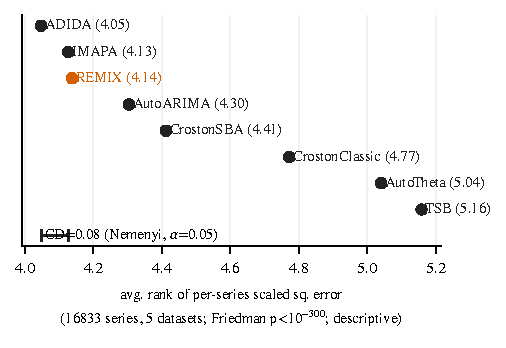
\includegraphics[width=0.93\linewidth]{figs/cd_diagram.pdf}
\caption{Average ranks of per-series scaled squared errors over the
16{,}833 series with complete saved row-level point predictions across
the five panels. The critical-difference bar is shown only for scale:
series, rather than datasets, are the blocks, so this is descriptive and
not a valid Friedman--Nemenyi test.}
\label{fig:cd}
\end{figure}

\subsection{Selection objective and efficiency}
\label{sec:criterion}\label{sec:efficiency}

The selector is not mathematically tied to pinball loss; it scores the
criterion supplied on the chronological validation tail. We use
item-averaged SPL because the target is a predictive distribution. The
best candidates are locally close, and a full cross-objective regret
matrix remains future work.

Joint selection takes $51$--$243$ seconds across the five panels,
excluding data loading, and covers 24 forecast candidates with one
deterministic EM/BIC search for the mixture on the fitting head. Final
estimation is analytic apart from low-dimensional group optimization;
selection and point prediction are deterministic, while probabilistic
bootstrap averaging uses the released fixed seed.

\subsection{Measured cost of every method}
\label{app:efficiency}

Table~\ref{tab:efficiency} reports instrumented wall-clock for every
method of Table~\ref{tab:prob} on Carparts (2{,}509 series), measured on
one CPU workstation in a single session with configurations unchanged.
The \EBB{} row includes its complete 24-candidate joint selection in
addition to the final fit ($B{=}20$) and five-quantile prediction; the
TSB-tuned row likewise includes its 25-candidate selection. No method
uses a GPU. Figure~\ref{fig:cost-accuracy} plots cost against mean SPL.

On the daily panels the official TweedieGP implementation was run in full
under the authors' released defaults (sparse variational GP with 200
inducing points and log-spaced initialization for series longer than 200
observations, all training points otherwise; Adam with learning rate
$0.1$; 50{,}000 predictive samples; median-demand scaling; restart on
numerical failure) and the authors' daily period. Online Retail
(3{,}649 series) completed with no failed fits at a per-series median of
$5.1$\,s; M5 (5{,}000 series, 1{,}294 training observations) completed
with no failed fits at a per-series median of $17.3$\,s, of which roughly
half is the 50{,}000-sample predictive draw over the 647-step external
span (the original protocol forecasts 28 steps), a protocol difference
rather than a method cost. Two caveats govern every timing in
Table~\ref{tab:efficiency}. First, all rows were measured on one machine
in one session, and absolute values are not comparable across platforms.
Second, \citet{damato2025} report $0.24$\,s per Carparts series on an M3
MacBook Pro; on our machine the released defaults give $1.89$\,s (single
thread, median of twelve series) and the paper-stated budget of 100
iterations gives $0.97$\,s, because the released code doubles the
iteration cap for Tweedie likelihoods on series with at most 500
observations.

\begin{table*}[t]
\centering
\caption{Instrumented wall-clock on Carparts, one machine, one session.
``Sel.''\ marks totals that include the method's own hyperparameter or
candidate selection. AutoARIMA/AutoTheta share one StatsForecast call
(split across the two); the five conformal wrappers share one
residual-pool fit (split across the five). Rows below the rule are
recorded from prior run metadata rather than re-timed: DeepState is a
full-panel GluonTS/MXNet run, Chronos-Bolt is zero-shot inference on a
500-series subsample, and DRP is a 500-series Online Retail subsample
(no Carparts run exists). All rows are CPU-only.}
\label{tab:efficiency}
\small
\setlength{\tabcolsep}{4.5pt}
\begin{tabular}{lrrccl}
\toprule
Method & Total (s) & s/series & Sel. & Runtime & Bit-repr.\\
\midrule
\EBB{} & 46.7 & 0.019 & yes & Python & Yes\\
TSB-tuned & 3.8 & 0.002 & yes & Python & No\\
CP wrappers (each) & 13.3 & 0.005 & no & Python & No\\
Tweedie-GLM & 37.3 & 0.015 & no & Python & No\\
iETS & 55.3 & 0.022 & no & R & No\\
AutoARIMA & 56.2 & 0.022 & no & Python & No\\
AutoTheta & 56.2 & 0.022 & no & Python & No\\
TweedieGP (12 workers) & 302.1 & 0.120 & no & Python/torch & No\\
\midrule
DeepState & 192.0 & 0.077 & no & Python/MXNet & No\\
Chronos-Bolt-small & 8.3 & 0.017 & no & Python/torch & No\\
DRP (Deep Renewal) & 1200.0 & 2.400 & no & Python/MXNet & No\\
\bottomrule
\end{tabular}
\end{table*}

\begin{table*}[t]
\centering
\caption{Walk-forward wall-clock per method and panel (seconds unless
marked in hours), covering every block of the protocol of
Table~\ref{tab:wfprob}: initialization, all per-block refits or updates,
and prediction. StatsForecast, conformal, and ACI rows run
single-process; TweedieGP runs its released code with twelve worker
processes; \EBB{} runs on one core and includes its initialization.
AutoARIMA and AutoTheta share one call. $^{\dagger}$Projected from the
measured $7{,}618$\,s full fit on the 5{,}000-series M5 sample at the
Online Retail cadence of one refit per four blocks ($24$ refits); at one
refit per block the projection is about $197$\,h. Neither was run.}
\label{tab:wfcost}
\small
\setlength{\tabcolsep}{5pt}
\begin{tabular}{lrrrrr}
\toprule
Method & Online Retail & Carparts & Auto & RAF & M5\\
\midrule
AutoARIMA & 1169 & 1.1\,h & 763 & 2.7\,h & ---\\
AutoTheta & 1169 & 1.1\,h & 763 & 2.7\,h & ---\\
iETS & 1795 & 270 & 213 & 1254 & ---\\
CP-ADIDA & --- & 9.6 & 4.4 & 38.0 & 465\\
ACI-ADIDA & 126 & 7.4 & 8.9 & 27.3 & 581\\
TweedieGP & 1.7\,h & 2686 & 2139 & 2.4\,h & $\approx$51\,h$^{\dagger}$\\
\midrule
\EBB{} & 22.4 & 3.4 & 3.6 & 13.5 & 36.6\\
ACI-\EBB{} & 52.3 & 4.2 & 4.8 & 13.3 & 217\\
\EBB{} (rule) & 22.4 & 3.4 & 4.8 & 13.5 & 217\\
\bottomrule
\end{tabular}
\end{table*}

\begin{figure}[t]
\centering
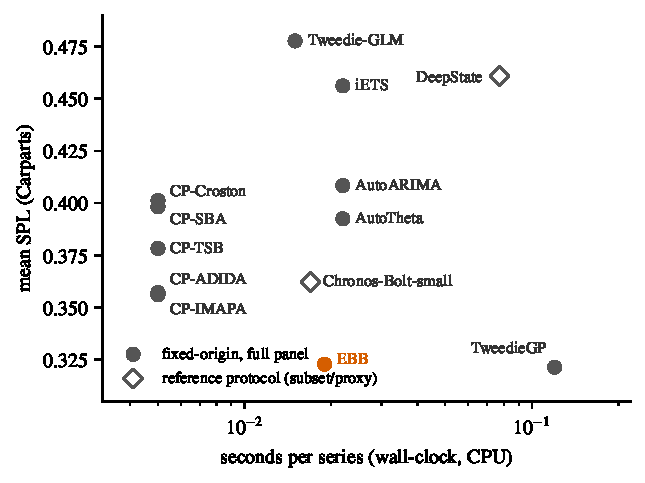
\includegraphics[width=0.95\linewidth]{figs/fig11_cost_accuracy_carparts.pdf}
\caption{Wall-clock cost per series against mean SPL on Carparts.
Filled circles are fixed-origin full-panel runs from
Table~\ref{tab:efficiency}; open diamonds are the reference points with
subset or proxy protocols. All methods run on CPU.}
\label{fig:cost-accuracy}
\end{figure}

\subsection{Controlled-study diagnostics}
\label{app:simulation-details}

In the length sweep used to isolate credibility leverage, the generator
holds $K=2$, 500 items per group, occurrence probabilities $0.05$ and
$0.80$, log-size centers three units apart, and $w=1$. The true
partition's pinball advantage falls monotonically from $1.53\%$ at
$T=12$ (median 4.5 positives per item) to $0.01\%$ at $T=400$ (median
154), with NLL, Brier, and log-size MSE following the same direction.
Across the main grid, the RMSE of $\hat\tau_g^2$ approximately doubles
as $w$ falls from $1.00$ to $0.90$ ($0.037\to0.144$ at $T=120$ and
$0.074\to0.149$ at $T=30$), directly measuring the resolution cost in
Proposition~\ref{prop:twosided}.

The generator centers the groups symmetrically around a fixed grand mean
so that increasing separation does not change total demand scale, and
every arm is evaluated through the same hurdle-lognormal predictive
representation under both likelihood-based proper scores and point
metrics. A four-arm ladder---single pool, true labels with estimated
hyperparameters, true labels with true hyperparameters, and the true
conditional law---checks the implementation; the true conditional law is
best on every metric in every cell.

\paragraph{Separation axis.} The grid above pools the three separations
$\{0.5,1,2\}$ of the original sweep, and the length sweep uses a single
separation of three; the envelope of Figure~\ref{fig:refinement-leverage}
therefore mixes separations. To resolve them we rerun the same generator
on a pre-registered grid: separation $\in\{0,0.25,0.5,1,2,3\}$ log-units
between adjacent group centers, $w\in\{1,0.95,0.90\}$, $T\in\{30,120\}$,
nine paired replicates per cell (seed 20260913), four groups of sixty
items, $\tau^2=0.15$, $\sigma^2=1$, occurrence spread in logit scaled
with the size separation as $0.8\min(\mathrm{sep},1)$ so that zero
separation removes structure from both blocks (a first pass held it fixed
at $0.8$; it is archived and superseded). Each cell records the true partition's paired pinball gain over a
single pool, the gain of the paper's mixture objective run on the same
panel, the median size-block credibility under the single pool, and the
share of item log-size variance explained by the true labels ($R^2$,
computed from the discounted item statistics so it includes sampling
noise). Two remedies for the learned mixture that already exist in the released
code are run as extra arms on the same panels: label sample-splitting
(labels from one interleaved half, hyperparameters from the other) and
credibility shrinkage of the group variance component, alone and
combined. Table~\ref{tab:sepsim} summarizes
the surface by separation and Table~\ref{tab:separation} reads it at the
real panels' coordinates. Real-panel $R^2$ uses the same statistic under
the learned mixture labels at the selected discount and under the
ADI/CV$^2$ taxonomy; we do not use the learned $\hat\tau_g^2$ as a scale
because it collapses to its floor under learned partitions
(Section~\ref{sec:leverage}). The simulation was run and summarized
before the real panels were placed.

\begin{table}[t]
\centering
\caption{Separation-resolved controlled study, averaged over the six
$(w,T)$ cells at each separation: true-label $R^2$, the true partition's
gain over a single pool, the learned mixture's gain, the same with label
sample-splitting and credibility shrinkage combined, and the median
number of components the mixture selects.}
\label{tab:sepsim}
\small
\setlength{\tabcolsep}{5pt}
\begin{tabular}{lrrrrr}
\toprule
Separation & $R^2$ & True (\%) & Learned (\%) & Learned+fix (\%) & $K$\\
\midrule
0 & 0.01 & +0.07 & -0.02 & -0.36 & 1\\
0.25 & 0.19 & +0.12 & -0.01 & -0.30 & 1\\
0.5 & 0.47 & +0.70 & -0.92 & -0.94 & 2\\
1 & 0.75 & +0.20 & -1.47 & -0.86 & 2\\
2 & 0.93 & -0.08 & -0.71 & -0.37 & 3\\
3 & 0.97 & -0.30 & -0.37 & -0.51 & 4\\
\bottomrule
\end{tabular}
\end{table}

\begin{table*}[t]
\centering
\caption{Real panels placed on the separation-resolved surface. $w$ is the
simulated discount matching the panel's selected one; $R^2$ is the
size-block separation under the learned partition and under the taxonomy,
and ``family $R^2$'' the true-label $R^2$ of the simulated family at the
panel's $\lambda^{(+)}$ ($T{=}120$). ``Room'' is the true partition's gain
interpolated along $\lambda^{(+)}$ within the matching $w$ at each length;
``sim.\ learned'' the learned mixture's gain at the same point
($T{=}120$); ``realized'' the panel's internal refinement gain
(Figure~\ref{fig:refinement-leverage}).}
\label{tab:separation}
\small
\setlength{\tabcolsep}{4.5pt}
\begin{tabular}{lrrrrrrrrr}
\toprule
Panel & $w$ & $\lambda^{(+)}$ & $R^2$ learned & $R^2$ tax. & family $R^2$ & Room $T{=}30$ & Room $T{=}120$ & Sim.\ learned & Realized\\
\midrule
Online Retail & 0.95 & 0.553 & 0.44 & 0.17 & 0.63 & -0.52 & +0.63 & -0.87 & -0.05\\
M5 & 0.95 & 0.841 & 0.79 & 0.30 & 0.86 & -0.34 & -0.45 & -1.21 & +0.58\\
Auto & 1 & 0.940 & 0.82 & 0.14 & 0.72 & -0.50 & -0.33 & -0.45 & -0.31\\
Carparts & 0.9 & 0.224 & 0.68 & 0.01 & 0.55 & +2.01 & +1.73 & -0.75 & -0.08\\
RAF & 1 & 0.917 & 0.95 & 0.09 & 0.62 & -0.48 & -0.41 & -0.58 & +0.03\\
\bottomrule
\end{tabular}
\end{table*}

